% ===========================================================================
%  TikuOS — TikuKits ML: Decision Tree for Embedded Systems
%  Beamer Presentation
% ===========================================================================
\documentclass[aspectratio=169, 10pt]{beamer}

% ---- Theme ----------------------------------------------------------------
\usetheme{Madrid}
\usecolortheme{whale}
\setbeamertemplate{navigation symbols}{}
\setbeamertemplate{footline}{%
  \leavevmode\hbox{%
    \begin{beamercolorbox}[wd=.33\paperwidth,ht=2.5ex,dp=1ex,center]{author in head/foot}%
      \usebeamerfont{author in head/foot}\insertshortauthor
    \end{beamercolorbox}%
    \begin{beamercolorbox}[wd=.34\paperwidth,ht=2.5ex,dp=1ex,center]{title in head/foot}%
      \usebeamerfont{title in head/foot}\insertshorttitle
    \end{beamercolorbox}%
    \begin{beamercolorbox}[wd=.33\paperwidth,ht=2.5ex,dp=1ex,right]{date in head/foot}%
      \usebeamerfont{date in head/foot}\insertshortdate{}\hspace*{2em}%
      \insertframenumber{}/\inserttotalframenumber\hspace*{2ex}
    \end{beamercolorbox}}%
  \vskip0pt%
}

% ---- Packages -------------------------------------------------------------
\usepackage{listings}
\usepackage{graphicx}
\usepackage{hyperref}
\usepackage{booktabs}
\usepackage{multirow}
\usepackage{tikz}
\usetikzlibrary{arrows.meta, positioning, shapes.geometric, calc,
                decorations.pathreplacing, fit}
\usepackage{amsmath}

% ---- Code listing style ---------------------------------------------------
\lstset{
  basicstyle=\ttfamily\scriptsize,
  keywordstyle=\color{blue}\bfseries,
  commentstyle=\color{gray},
  stringstyle=\color{red!70!black},
  showstringspaces=false,
  breaklines=true,
  frame=single,
  rulecolor=\color{black!30},
  backgroundcolor=\color{blue!3},
  tabsize=4,
}
\lstdefinestyle{cstyle}{
  language=C,
  morekeywords={uint8_t,uint16_t,uint32_t,int32_t,int64_t,
                tiku_kits_ml_elem_t,
                TIKU_KITS_ML_OK,TIKU_KITS_ML_ERR_NULL,
                TIKU_KITS_ML_ERR_SIZE,TIKU_KITS_ML_ERR_PARAM,
                TIKU_KITS_ML_DTREE_MAX_NODES,
                TIKU_KITS_ML_DTREE_MAX_FEATURES,
                TIKU_KITS_ML_DTREE_LEAF,
                NULL},
}

% ---- Metadata -------------------------------------------------------------
\title[TikuKits ML]{TikuKits ML: Decision Tree for Embedded Systems}
\subtitle{Simple. Ubiquitous. Intelligence, Everywhere.}
\author[Ambuj Varshney]{Ambuj Varshney \\ \texttt{ambuj@tiku-os.org}}
\date{\today}

% ===========================================================================
\begin{document}

% ---------------------------------------------------------------------------
\begin{frame}
\titlepage
\end{frame}

% ---------------------------------------------------------------------------
\begin{frame}{Outline}
\tableofcontents
\end{frame}

% ===========================================================================
\section{Motivation}
% ===========================================================================

\begin{frame}{Why Decision Trees on MCUs?}
\begin{columns}[T]
\begin{column}{0.48\textwidth}
\begin{block}{Embedded Use Cases}
\begin{itemize}
  \item \textbf{Multi-class classification} --- temperature zones, fault types
  \item \textbf{Interpretable rules} --- each node is a simple threshold
  \item \textbf{Fast inference} --- O(depth) comparisons, no multiply
  \item \textbf{Confidence scores} --- leaf confidence for triage
\end{itemize}
\end{block}

\begin{block}{Constraints}
\begin{itemize}
  \item No FPU (16-bit MSP430)
  \item No heap allocation
  \item Limited RAM (2--8\,KB)
  \item Every $\mu$J counts
\end{itemize}
\end{block}
\end{column}

\begin{column}{0.48\textwidth}
\begin{center}
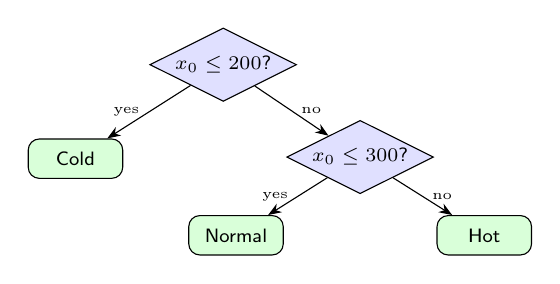
\begin{tikzpicture}[
    >=Stealth, node distance=0.5cm,
    decision/.style={draw, diamond, aspect=2, inner sep=1pt,
                     font=\scriptsize\sffamily, fill=blue!12},
    leaf/.style={draw, rounded corners, minimum height=0.5cm,
                 font=\scriptsize\sffamily, fill=green!15,
                 text centered, minimum width=1.2cm}
  ]
  \node[decision] (n0) {$x_0 \leq 200$?};
  \node[leaf, below left=0.7cm and 0.8cm of n0] (l0) {Cold};
  \node[decision, below right=0.7cm and 0.8cm of n0] (n1) {$x_0 \leq 300$?};
  \node[leaf, below left=0.5cm and 0.5cm of n1] (l1) {Normal};
  \node[leaf, below right=0.5cm and 0.5cm of n1] (l2) {Hot};

  \draw[->] (n0) -- node[left, font=\tiny] {yes} (l0);
  \draw[->] (n0) -- node[right, font=\tiny] {no} (n1);
  \draw[->] (n1) -- node[left, font=\tiny] {yes} (l1);
  \draw[->] (n1) -- node[right, font=\tiny] {no} (l2);
\end{tikzpicture}
\end{center}

\vspace{0.5em}
\begin{alertblock}{Design Goal}
Pre-built decision trees on MCU: array-based node storage,
\textbf{O(depth)} inference with only integer comparisons.
No training on-device --- train offline, deploy the tree.
\end{alertblock}
\end{column}
\end{columns}
\end{frame}

% ===========================================================================
\section{Algorithm Theory}
% ===========================================================================

\begin{frame}{Decision Tree Inference}
\begin{columns}[T]
\begin{column}{0.48\textwidth}
\textbf{Tree structure:}
\begin{itemize}
  \item Each internal node tests one feature against a threshold
  \item Left child: $x[\text{feature}] \leq \text{threshold}$
  \item Right child: $x[\text{feature}] > \text{threshold}$
  \item Leaf nodes store the predicted class
\end{itemize}

\vspace{0.5em}
\textbf{Inference algorithm:}
\begin{enumerate}
  \item Start at root node (index 0)
  \item Compare $x[\text{feature\_index}]$ with threshold
  \item Follow left or right child
  \item Repeat until a leaf node is reached
  \item Return the leaf's class label
\end{enumerate}

\vspace{0.5em}
\textbf{Complexity:} O(depth) comparisons per sample.\\
No multiplications, no accumulations.
\end{column}

\begin{column}{0.48\textwidth}
\textbf{Array-based storage:}
\begin{center}
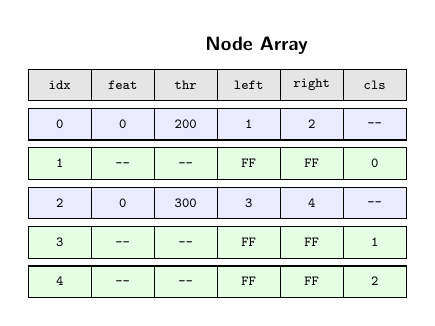
\begin{tikzpicture}[
    >=Stealth,
    cell/.style={draw, minimum width=0.8cm, minimum height=0.4cm,
                 font=\tiny\ttfamily}
  ]
  \node[font=\scriptsize\sffamily\bfseries] at (2.5, 2.8) {Node Array};

  % Headers
  \node[cell, fill=gray!20] at (0, 2.3) {idx};
  \node[cell, fill=gray!20] at (0.8, 2.3) {feat};
  \node[cell, fill=gray!20] at (1.6, 2.3) {thr};
  \node[cell, fill=gray!20] at (2.4, 2.3) {left};
  \node[cell, fill=gray!20] at (3.2, 2.3) {right};
  \node[cell, fill=gray!20] at (4.0, 2.3) {cls};

  % Node 0 (root)
  \node[cell, fill=blue!8] at (0, 1.8) {0};
  \node[cell, fill=blue!8] at (0.8, 1.8) {0};
  \node[cell, fill=blue!8] at (1.6, 1.8) {200};
  \node[cell, fill=blue!8] at (2.4, 1.8) {1};
  \node[cell, fill=blue!8] at (3.2, 1.8) {2};
  \node[cell, fill=blue!8] at (4.0, 1.8) {--};

  % Node 1 (leaf: cold)
  \node[cell, fill=green!10] at (0, 1.3) {1};
  \node[cell, fill=green!10] at (0.8, 1.3) {--};
  \node[cell, fill=green!10] at (1.6, 1.3) {--};
  \node[cell, fill=green!10] at (2.4, 1.3) {FF};
  \node[cell, fill=green!10] at (3.2, 1.3) {FF};
  \node[cell, fill=green!10] at (4.0, 1.3) {0};

  % Node 2 (internal)
  \node[cell, fill=blue!8] at (0, 0.8) {2};
  \node[cell, fill=blue!8] at (0.8, 0.8) {0};
  \node[cell, fill=blue!8] at (1.6, 0.8) {300};
  \node[cell, fill=blue!8] at (2.4, 0.8) {3};
  \node[cell, fill=blue!8] at (3.2, 0.8) {4};
  \node[cell, fill=blue!8] at (4.0, 0.8) {--};

  % Nodes 3,4 (leaves)
  \node[cell, fill=green!10] at (0, 0.3) {3};
  \node[cell, fill=green!10] at (0.8, 0.3) {--};
  \node[cell, fill=green!10] at (1.6, 0.3) {--};
  \node[cell, fill=green!10] at (2.4, 0.3) {FF};
  \node[cell, fill=green!10] at (3.2, 0.3) {FF};
  \node[cell, fill=green!10] at (4.0, 0.3) {1};

  \node[cell, fill=green!10] at (0, -0.2) {4};
  \node[cell, fill=green!10] at (0.8, -0.2) {--};
  \node[cell, fill=green!10] at (1.6, -0.2) {--};
  \node[cell, fill=green!10] at (2.4, -0.2) {FF};
  \node[cell, fill=green!10] at (3.2, -0.2) {FF};
  \node[cell, fill=green!10] at (4.0, -0.2) {2};
\end{tikzpicture}
\end{center}

\vspace{0.3em}
\begin{block}{Leaf Sentinel}
\texttt{left = right = 0xFF} marks a leaf node.
No pointers needed --- array indices only.
\end{block}
\end{column}
\end{columns}
\end{frame}

% ===========================================================================
\section{Data Structure}
% ===========================================================================

\begin{frame}[fragile]{The \texttt{tiku\_kits\_ml\_dtree} Structure}
\begin{columns}[T]
\begin{column}{0.48\textwidth}
\begin{lstlisting}[style=cstyle,
  title={Node and tree structures}]
struct tiku_kits_ml_dtree_node {
    int32_t  threshold;
    uint8_t  feature_index;
    uint8_t  left;    /* or 0xFF = leaf */
    uint8_t  right;   /* or 0xFF = leaf */
    uint8_t  class_label;
};

struct tiku_kits_ml_dtree {
    struct tiku_kits_ml_dtree_node
        nodes[TIKU_KITS_ML_DTREE_MAX_NODES];
    uint8_t n_nodes;
    uint8_t n_features;
    uint8_t shift;
};
\end{lstlisting}

\textbf{Memory footprint:}\\
$31 \times 8 + 3 = 251$ bytes (default config).
\end{column}

\begin{column}{0.48\textwidth}
\begin{lstlisting}[style=cstyle,
  title={Configuration macros}]
/* Max nodes (depth-4 complete tree) */
#ifndef TIKU_KITS_ML_DTREE_MAX_NODES
#define TIKU_KITS_ML_DTREE_MAX_NODES 31
#endif

/* Max input features */
#ifndef TIKU_KITS_ML_DTREE_MAX_FEATURES
#define TIKU_KITS_ML_DTREE_MAX_FEATURES 8
#endif

/* Leaf sentinel value */
#define TIKU_KITS_ML_DTREE_LEAF 0xFF
\end{lstlisting}

\vspace{0.3em}
\begin{block}{Design Trade-off}
31 nodes supports a depth-4 tree (15 internal + 16 leaves).
Increase \texttt{MAX\_NODES} for deeper trees at cost of RAM.
\end{block}
\end{column}
\end{columns}
\end{frame}

% ===========================================================================
\section{API Reference}
% ===========================================================================

\begin{frame}[fragile]{Complete API}
\begin{table}
\centering
\small
\begin{tabular}{@{}lp{8cm}@{}}
\toprule
\textbf{Function} & \textbf{Description} \\
\midrule
\texttt{tiku\_kits\_ml\_dtree\_init(dt, nf, sh)}
  & Initialize model with \texttt{nf} features, Q-format \texttt{sh} \\
\texttt{tiku\_kits\_ml\_dtree\_reset(dt)}
  & Clear all nodes \\
\texttt{tiku\_kits\_ml\_dtree\_set\_tree(dt, nodes, n)}
  & Load pre-built tree with validation \\
\midrule
\texttt{tiku\_kits\_ml\_dtree\_predict(dt, x, \&result)}
  & Return class label at reached leaf \\
\texttt{tiku\_kits\_ml\_dtree\_predict\_proba(dt, x, \&conf)}
  & Return leaf's confidence value in Q(shift) \\
\midrule
\texttt{tiku\_kits\_ml\_dtree\_get\_tree(dt, out, \&n)}
  & Export the loaded tree \\
\texttt{tiku\_kits\_ml\_dtree\_node\_count(dt)}
  & Number of loaded nodes \\
\texttt{tiku\_kits\_ml\_dtree\_depth(dt)}
  & Actual depth of the tree \\
\bottomrule
\end{tabular}
\end{table}

\vspace{0.3em}
\begin{alertblock}{Pre-Built Trees Only}
Decision trees are \textbf{not trained} on the MCU. Build the tree offline
(e.g.\ scikit-learn), export as a node array, and load with
\texttt{set\_tree()}. The \texttt{set\_tree()} function validates all
child indices and feature indices for safety.
\end{alertblock}
\end{frame}

% ===========================================================================
\section{Examples}
% ===========================================================================

\begin{frame}[fragile]{Example 1: Temperature Zone Classification}
\begin{lstlisting}[style=cstyle,
  title={examples/example\_ml\_dtree.c --- 3-class temperature zones}]
struct tiku_kits_ml_dtree dt;
uint8_t result;

tiku_kits_ml_dtree_init(&dt, 1, 8);   /* 1 feature, Q8 */

/* Build tree: cold(<200) / normal(200-300) / hot(>300) */
struct tiku_kits_ml_dtree_node tree[] = {
    /* [0] root: x[0] <= 200? */
    { .threshold = 200, .feature_index = 0, .left = 1, .right = 2,
      .class_label = 0 },
    /* [1] leaf: cold (class 0) */
    { .threshold = 230, .feature_index = 0,
      .left = 0xFF, .right = 0xFF, .class_label = 0 },
    /* [2] internal: x[0] <= 300? */
    { .threshold = 300, .feature_index = 0, .left = 3, .right = 4,
      .class_label = 0 },
    /* [3] leaf: normal (class 1) */
    { .threshold = 240, .feature_index = 0,
      .left = 0xFF, .right = 0xFF, .class_label = 1 },
    /* [4] leaf: hot (class 2) */
    { .threshold = 250, .feature_index = 0,
      .left = 0xFF, .right = 0xFF, .class_label = 2 },
};

tiku_kits_ml_dtree_set_tree(&dt, tree, 5);

tiku_kits_ml_elem_t temp = 250;
tiku_kits_ml_dtree_predict(&dt, &temp, &result);  /* result = 1 (normal) */
\end{lstlisting}
\end{frame}

% ---------------------------------------------------------------------------
\begin{frame}[fragile]{Example 2: Confidence-Aware Triage}
\begin{columns}[T]
\begin{column}{0.52\textwidth}
\begin{lstlisting}[style=cstyle,
  title={Using predict\_proba for triage}]
struct tiku_kits_ml_dtree dt;
uint8_t result;
int32_t confidence;

/* ... init and set_tree ... */

tiku_kits_ml_elem_t x[] = {250};

/* Get class + confidence */
tiku_kits_ml_dtree_predict(&dt,
    x, &result);
tiku_kits_ml_dtree_predict_proba(&dt,
    x, &confidence);

/* Confidence-aware decision */
if (confidence > 200) {
    /* High confidence: act */
    set_alarm(result);
} else {
    /* Low confidence: defer */
    request_more_samples();
}
\end{lstlisting}
\end{column}

\begin{column}{0.44\textwidth}
\begin{center}
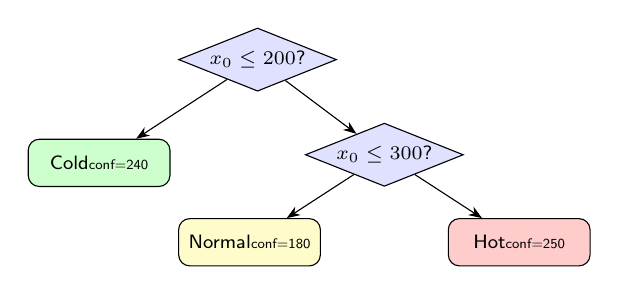
\begin{tikzpicture}[
    >=Stealth, node distance=0.4cm,
    decision/.style={draw, diamond, aspect=2.5, inner sep=1pt,
                     font=\scriptsize\sffamily, fill=blue!12},
    leaf/.style={draw, rounded corners, minimum height=0.6cm,
                 font=\scriptsize\sffamily, text centered,
                 minimum width=1.8cm}
  ]
  \node[decision] (n0) {$x_0 \leq 200$?};
  \node[leaf, fill=green!20, below left=0.8cm and 0.6cm of n0]
    (l0) {Cold\\{\tiny conf=240}};
  \node[decision, below right=0.8cm and 0.6cm of n0] (n1) {$x_0 \leq 300$?};
  \node[leaf, fill=yellow!20, below left=0.6cm and 0.3cm of n1]
    (l1) {Normal\\{\tiny conf=180}};
  \node[leaf, fill=red!20, below right=0.6cm and 0.3cm of n1]
    (l2) {Hot\\{\tiny conf=250}};

  \draw[->] (n0) -- (l0);
  \draw[->] (n0) -- (n1);
  \draw[->] (n1) -- (l1);
  \draw[->] (n1) -- (l2);
\end{tikzpicture}
\end{center}

\vspace{0.5em}
\begin{block}{Leaf Confidence}
The \texttt{threshold} field of leaf nodes stores a
confidence value (set during offline training).
\texttt{predict\_proba()} returns this value.
\end{block}
\end{column}
\end{columns}
\end{frame}

% ===========================================================================
\section{Test Suite}
% ===========================================================================

\begin{frame}{Test Cases Overview}
\begin{table}
\centering
\small
\begin{tabular}{@{}clp{7cm}@{}}
\toprule
\textbf{\#} & \textbf{Test Function} & \textbf{What It Verifies} \\
\midrule
1 & \texttt{test\_kits\_ml\_dtree\_init}
  & Proper initialization, parameter validation \\
2 & \texttt{test\_kits\_ml\_dtree\_simple\_tree}
  & Single-split binary classification \\
3 & \texttt{test\_kits\_ml\_dtree\_multi\_feature}
  & Tree with multiple feature splits \\
4 & \texttt{test\_kits\_ml\_dtree\_depth}
  & Tree depth calculation \\
5 & \texttt{test\_kits\_ml\_dtree\_predict\_proba}
  & Confidence value extraction from leaves \\
6 & \texttt{test\_kits\_ml\_dtree\_boundary}
  & Exact-threshold boundary behavior \\
7 & \texttt{test\_kits\_ml\_dtree\_get\_tree}
  & Tree export round-trip \\
8 & \texttt{test\_kits\_ml\_dtree\_reset}
  & Reset clears all nodes \\
9 & \texttt{test\_kits\_ml\_dtree\_null\_inputs}
  & All functions reject NULL with ERR\_NULL \\
\bottomrule
\end{tabular}
\end{table}
\end{frame}

% ===========================================================================
\section{Summary}
% ===========================================================================

\begin{frame}{Summary}
\begin{columns}[T]
\begin{column}{0.48\textwidth}
\begin{block}{What We Built}
\begin{itemize}
  \item Pre-built decision tree classifier
  \item Array-based node storage (no pointers)
  \item O(depth) inference --- comparisons only
  \item 251 bytes state (default 31 nodes)
  \item Confidence output via leaf threshold
\end{itemize}
\end{block}

\begin{block}{Key Design Choices}
\begin{itemize}
  \item Sentinel \texttt{0xFF} marks leaf nodes
  \item \texttt{set\_tree()} validates all indices
  \item No on-device training (deploy offline trees)
  \item Multi-class support (any number of classes)
\end{itemize}
\end{block}
\end{column}

\begin{column}{0.48\textwidth}
\begin{block}{Use Cases}
\begin{itemize}
  \item Temperature zone classification
  \item Vibration fault type detection
  \item Multi-sensor triage decisions
  \item Confidence-aware alerting
\end{itemize}
\end{block}

\begin{block}{Files}
\scriptsize
\begin{tabular}{@{}lp{4.5cm}@{}}
Header: & \texttt{ml/classification/tiku\_kits\_ml\_dtree.h} \\
Source: & \texttt{ml/classification/tiku\_kits\_ml\_dtree.c} \\
Tests: & \texttt{tests/ml/test\_kits\_ml\_dtree.c} \\
Example: & \texttt{examples/example\_ml\_dtree.c} \\
\end{tabular}
\end{block}
\end{column}
\end{columns}
\end{frame}

% ---------------------------------------------------------------------------
\begin{frame}{Thank You}
\begin{center}
\Large\textbf{TikuKits ML: Decision Tree}\\[0.5em]
\normalsize Integer-Only Machine Learning for Physical AI Endpoints\\[1.5em]

\begin{tabular}{rl}
  Repository: & \url{https://github.com/tikuos/tikuOS} \\
  License:    & Apache 2.0 \\
  Common:     & \texttt{tikukits/ml/tiku\_kits\_ml.h} \\
  Header:     & \texttt{tikukits/ml/classification/tiku\_kits\_ml\_dtree.h} \\
  Source:     & \texttt{tikukits/ml/classification/tiku\_kits\_ml\_dtree.c} \\
  Tests:      & \texttt{tikukits/tests/ml/test\_kits\_ml\_dtree.c} \\
  Examples:   & \texttt{tikukits/examples/example\_ml\_dtree.c} \\
\end{tabular}
\end{center}
\end{frame}

\end{document}
